\subsection{Fitting a GP with Pyro}
All code for this task and the next is contained in the \texttt{function\_fitting.ipynb} notebook. We have implemented the required NUTS sampling, and the scatter plot of $p(\theta | \mathcal{D})$ which can be seen in Figure \ref{fig:p_theta}.
\begin{figure}[h]
\centering
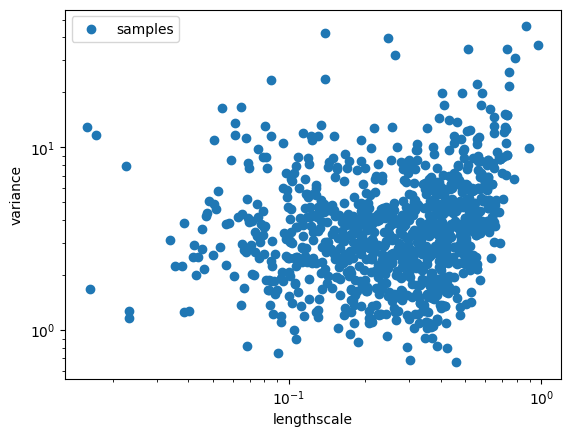
\includegraphics[width=0.5\linewidth]{images/p_theta.png}
\setlength{\belowcaptionskip}{-10pt}
\caption{Scatter plot showing 500 sampled from $p(\theta | \mathcal{D})$}
\label{fig:p_theta}
\end{figure}

We used Arviz to gauge the quality of our samples, which gave us the plots that can be seen in Figure \ref{fig:arviz_old}. It also told us that our effective bulk sample size is $249$ and $287$ for the \texttt{lengthscale} and \texttt{variance} parameters, respectively. With such few points in the dataset, having half of the samples be good seems to indicate a relatively high quality. However, the quality of the approximation is obviously not very good, as the number of points is not large enough to sufficiently capture the entire signal of the function. Any human asked to approximate the function given only the five points in $\mathcal{D}$ would come up with something very similar to what we find in our plot of $p(f^*|x^*,\mathcal{D})$ in Figure \ref{fig:f_star}.

\begin{figure}[h]
\centering
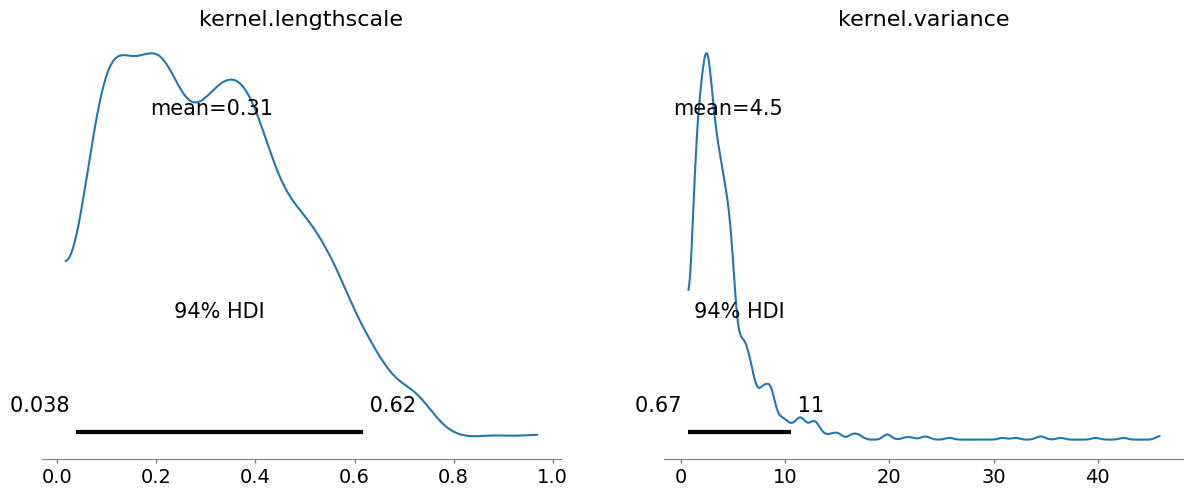
\includegraphics[width=0.75\linewidth]{images/arviz_single_0.png}\\
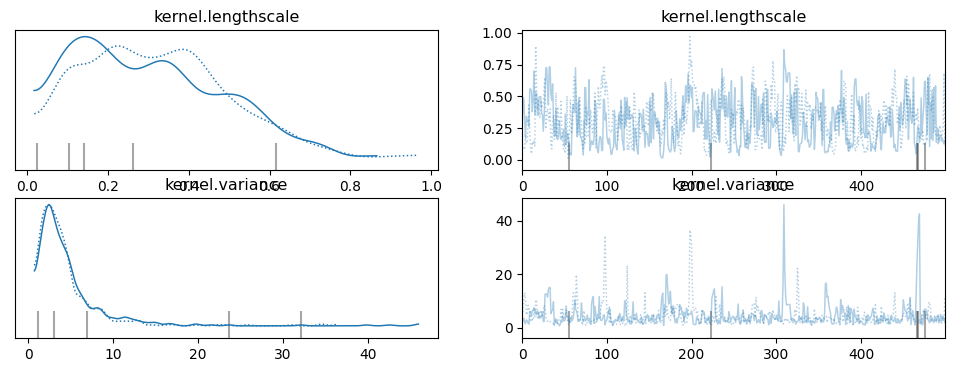
\includegraphics[width=0.75\linewidth]{images/arviz_single_1.png}
\setlength{\belowcaptionskip}{-10pt}
\caption{Arviz plots of the results.}
\label{fig:arviz_old}
\end{figure}


\begin{figure}[h]
\centering
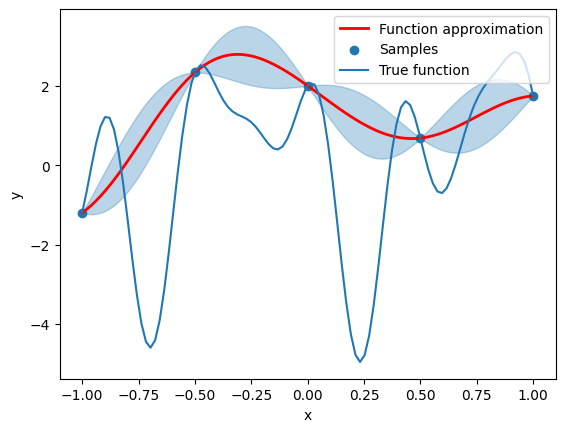
\includegraphics[width=0.5\linewidth]{images/f_star.png}
\setlength{\belowcaptionskip}{-10pt}
\caption{Plot visualising $p(f^*|x^*, \mathcal{D})$}
\label{fig:f_star}
\end{figure}
